\chapter{Primitive Detection Algorithms}

\begin{figure}[ht!]
    \centering
    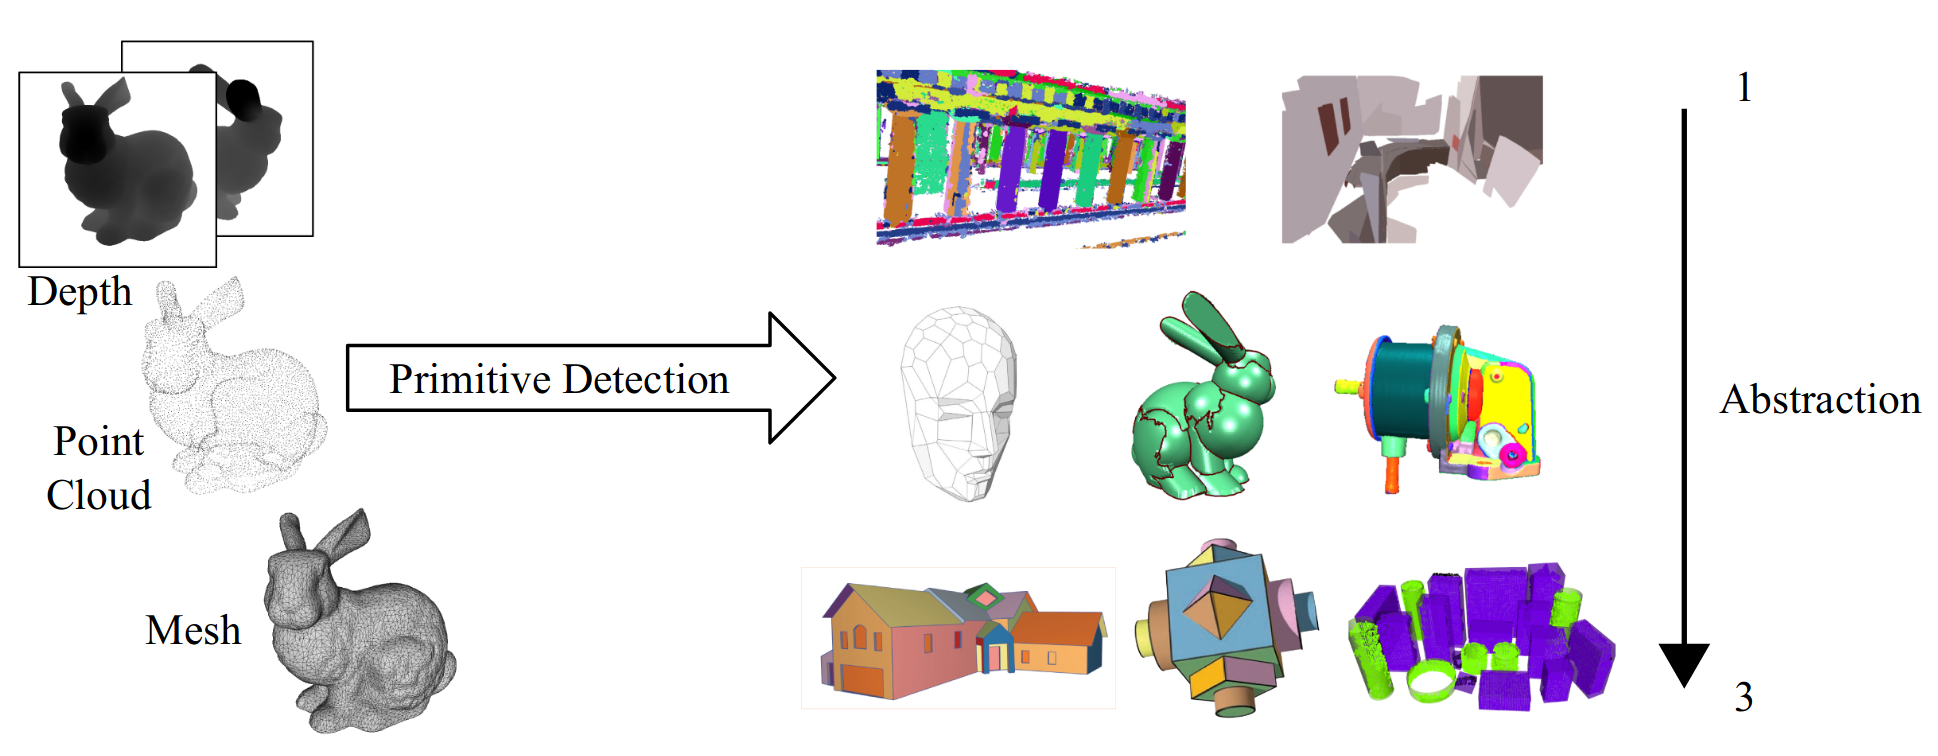
\includegraphics[width=\linewidth]{images/primitive_detection}
    \caption{Process of detecting primitives}
    \label{fig:primitive_detection}
\end{figure}
Primitive detection is a well-established area in computer vision that aims to detect simple geometric shapes
like planes, spheres, cylinders, or cones a given input data.
These methods are model-fitting algorithms that identify the most likely model that fits a subset of the input data.
The result of these algorithms is a set of parameters that describe the detected shape.
These shapes are an abstraction of the input data, offering a simplified compact representation of the data,
allowing for higher performance and the ability to perform higher-level tasks such as object recognition or scene reconstruction.
The input data representation varies by algorithm, with the most common types being:
\begin{itemize}
    \item \textbf{Point Clouds:} A set of 3D points in space representing the sampled surface of the real-world
    \item \textbf{Depth Images:} A 2D image where each pixel represents the distance to the camera, typically obtained from depth sensors
    \item \textbf{Image Sequences:} A sequence of 2D images from different viewpoints that are typically first convert to a point cloud or depth image for further processing, further discussed in section~\ref{sec:technical-background-depth-from-motion}
    \item \textbf{Meshes:} A polygonal representation of surfaces, consisting of vertices, edges, and faces, typically generated from surface reconstruction algorithms. Not further considered in this thesis. \cite{kaiser_survey_2019}
\end{itemize}

This chapter provides an overview of the most common primitive detection algorithms by categorizing them based on their underlying methodology.
The chapter then compares the two most widely used base methodologies,
the Hough Transform and the Random Sample Consensus (RANSAC) algorithm.


\section{Categorization}
\citeauthor{kaiser_survey_2019}~\cite{kaiser_survey_2019} reviewed over 70 detection algorithms, evaluating them based on their input/output data types,
underlying methodology, supported primitive types, context of application and provides a rating for multiple criteria.
The authors categorize the underlying methodology of the algorithms into three categories:
\begin{itemize}
    \item \textbf{Stochastic:} algorithms that use random sampling to detect primitives, such as RANSAC
    \item \textbf{Parameter Space:} algorithms that use a parameter space to detect primitives, such as the Hough Transform
    \item \textbf{Other techniques}, for example primitive-driven region growing
\end{itemize}

The following sections provide an overview of the most common algorithms in each category.

\subsection{RANSAC (Stochastic)}
The Random Sample Consensus (RANSAC) algorithm is a widely used stochastic model parameter estimation
algorithm first introduced in~\citeyear{fischler_random_1981}
by~\citeauthor{fischler_random_1981}~\cite{fischler_random_1981}.
"The basic principle of the algorithm is to try many possible randomized models that could fit
the data and evaluate how good this model is in order to find a consensus,
i.e.\ an agreement of most of the data samples."~\parencite{kaiser_survey_2019}

For a given shape that requires $n$ points to be defined, RANSAC follows the following steps to detect the shape
in a set of data points $P$~\parencite{fischler_random_1981}:
\begin{enumerate}
    \item Randomly select a subset $S1$ of $n$ data points from $P$
    \item Fit the model $M1$ to the selected points
    \item Determine if the subset of inliers $S1^*$ of $P$ that fit the model $M1$ within a predefined tolerance, this is called the consensus set
    \item If size of the consensus set $|S1^*|$ is greater than a predefined threshold $t$, re-fit the model to $S1^*$, resulting in new model $M1^*$
    \item If size of the consensus set $|S1^*|$ is smaller than a predefined threshold $t$, repeat until a model with a consensus set of size $t$ is found or a predefined number of iterations is reached
\end{enumerate}

The algorithm has 3 main parameters that need to be set:
\begin{itemize}
    \item \textbf{Error tolernace:} the distance between a data point and the model under which the data point is considered an inlier
    \item \textbf{Threshold $t$:} the number of inliers required to consider a model valid
    \item \textbf{Number of iterations:} the number of times the algorithm will try to find a model with a consensus set of size $t$
\end{itemize}


\subsection{Hough Transform (Parameter Space)}
The Hough transform introduced in~\citeyear{hough_method_1962} by \citeauthor{hough_method_1962}~\parencite{hough_method_1962} creates a voting space based on parameters where similar shapes overlap.
This space is quantized into uniform sections, and each data point votes for the shapes it aligns with~\parencite{duda_use_1972}.
After all data points have voted, the parameters with the highest votes reveal the shape that most accurately fits the input data.
%todo go into more detail

\subsection{Primitive-driven Region Growing}

\section{Choosing an algorithm: Hough Transform vs RANSAC}

\cite{kaiser_survey_2019} lists over 70 detection algorithms, many of which are specialized for specific contexts.
However, as this thesis aims to develop an end to end implementation for detecting primitives using
a smartphone camera and rendering the detected primitives in AR, without focusing on a specific context,
algorithms that are widely used and applicable to a wide range of applications will be considered.
Both the Hough Transform and the Random Sample Consensus (RANSAC) algorithm stand out as the
most widely used methodologies in the field of primitive detection~\parencite{schnabel_efficient_2007}.
This section provides a comparison of these two methodologies and a decision on which algorithm to use for the implementation.
%todo

In general, the performance of both algorithms varies based on the context of the application.
With optimizations, both algorithms are suitable for a wide range of applications, as seen in the following example applications.
The Hough Transform is more computationally expensive than RANSAC~\parencite{kaiser_survey_2019}.
\cite{tarsha-kurdi_hough-transform_2007} found that its processing time is negligible in comparison to the Hough Transform.
RANSAC is also more robust to noise and outliers~\parencite{kaiser_survey_2019}.
It is also simpler and therefore easier to extend and adapt to different contexts~\parencite{tarsha-kurdi_hough-transform_2007, kaiser_survey_2019}.
The main drawback of RANSAC is that results are not repeatable, as the algorithm is based on random sampling~\parencite{kaiser_survey_2019}.


\paragraph{Application 1:}
\cite{tarsha-kurdi_hough-transform_2007} analyzed the application of detecting building
roofs as planes in 3D Lidar scans of cityscapes, and found that by default both RANSAC and Hough-Transform yield similar,
insufficient results for their use-case.
“That can be explained by the use of a pure mathematical principle,
without taking into account the particularity of the building Lidar data. […] That is why
[they] may detect a set of points which represents several roof planes or which belongs to several planes.”
They also had difficulties to determine the parameters of Hough Transform,
as the optimal values vary based on the characteristics of the point cloud.
Motivated by RANSACS rapidity they investigated extending the RANSAC algorithm and with their improvements
found that it produces satisfying results.

As apparent from the examples, both the Hough Transform and RANSAC are suitable algorithms for the detection of primitives.
However, the Hough Transform is more computationally expensive, harder to tune for specific contexts and less robust to noise and outliers.
RANSAC also has a publicly available reference implementation in C\texttt{++} by~\parencite{schnabel_efficient_2007},
which is e.g.\ used in the open source tool CloudCompare~\parencite{daniel_girardeau-montaut_cloudcompare_nodate} and can therefore be
easily tested on ones own pointclouds without the need to write custom code, useful for evaluation, as can later be seen in chapter~\ref{ch:evaluation}.
